%! suppress = Makeatletter
%! suppress = TooLargeSection
%! suppress = MissingLabel
\documentclass{article}

% Fields
\usepackage{geometry}
\geometry{top=25mm}
\geometry{bottom=35mm}
\geometry{left=20mm}
\geometry{right=20mm}
% ------------------------------------------------

% Graphics
\usepackage{color}
\usepackage{tabularx}
\usepackage{tikz}
\usepackage{blkarray}
\usepackage{graphicx}
% ------------------------------------------------

% Math
\usepackage{amsmath, amsfonts}
\usepackage{amssymb}
\usepackage{proof}
\usepackage{mathrsfs}
% Crossed-out symbols
% https://tex.stackexchange.com/questions/75525/how-to-write-crossed-out-math-in-latex
\usepackage[makeroom]{cancel}
\usepackage{mathtools}
% ------------------------------------------------

% Additional font sizes
% https://www.overleaf.com/learn/latex/Questions/How_do_I_adjust_the_font_size%3F
\usepackage{moresize}
% Additional colors
% https://www.overleaf.com/learn/latex/Using_colours_in_LaTeX
\usepackage{xcolor}
% \texttimes
\usepackage{textcomp}
% ------------------------------------------------

% Language
\usepackage[utf8] {inputenc}
\usepackage[T2A] {fontenc}
\usepackage[english, russian] {babel}
\usepackage{indentfirst, verbatim}
\usetikzlibrary{cd, babel}
% ------------------------------------------------

% Fonts
\usepackage{stmaryrd}
\usepackage{cmbright}
\usepackage{wasysym}
% ------------------------------------------------

% Code
% https://tex.stackexchange.com/questions/99475/how-to-invoke-latex-with-the-shell-escape-flag-in-texstudio-former-texmakerx
% Colored, requires --shell-escape compiling option
% \usepackage{minted}
% \setminted{xleftmargin=\parindent, autogobble, escapeinside=\#\#}
\usepackage{listings}
% ------------------------------------------------

% Custom envs
% https://tex.stackexchange.com/questions/371286/draw-a-horizontal-line-in-latex
\newenvironment{proof}{\subparagraph{\hspace{-1em}Решение:\newline}}{\par\noindent\rule{\textwidth}{0.4pt}}
% ------------------------------------------------

% Custom commands
\newcommand{\comb}[1]{\mathbf{#1}}
\newcommand{\step}{\rightsquigarrow}
\newcommand{\term}[1]{\mathbf{#1}}
\newcommand{\ap}{~}
\newcommand{\termdef}{\coloneqq}
\newcommand{\subst}[3]{\left[#2 \mapsto #3 \right] #1}
\newcommand{\eqbeta}{=_\beta}
\newcommand{\eqeta}{=_\eta}
\def\multiset#1#2{\ensuremath{\left(\kern-.3em\left(\genfrac{}{}{0pt}{}{#1}{#2}\right)\kern-.3em\right)}}
% ------------------------------------------------

% Head
\usepackage{fancybox,fancyhdr}
\usepackage{hyperref}
\pagestyle{fancy}
\fancyhead[R]{Максим Васильев (285800)} % TODO введите ваше имя
\fancyhead[L]{ИТМО MSE, ДМ 2023, Дз 11}
% ------------------------------------------------

% Numbering
% https://tex.stackexchange.com/questions/80113/hide-section-numbers-but-keep-numbering
\makeatletter
\renewcommand\thesubsection{Блок \@arabic\c@subsection.\hspace{-0.8em}}
\renewcommand\thesubsubsection{Задание \@arabic\c@subsection.\@arabic\c@subsubsection\hspace{-0.8em}}
% https://tex.stackexchange.com/questions/327689/numbering-subsubsections-with-letters
\renewcommand\theparagraph{\alph{paragraph})\hspace{-0.8em}}
% https://tex.stackexchange.com/questions/129208/numbering-paragraphs-in-latex
\setcounter{secnumdepth}{4}
\makeatother
% ------------------------------------------------

\begin{document}
\begin{enumerate}

    \item \textit{(1 балл)} Верно ли, что если в простом графе $G$ существует эйлеров цикл, то в нем существует и гамильтонов цикл? Верно ли обратное утверждение, а именно, что если в простом графе существует гамильтонов цикл, то в нем существует и эйлеров цикл?
    
    \textbf{Решение}:

    Первое утверждение не верно, потому что можно придумать контрпример: пусть есть граф, в котором существует эйлеров цикл. Добавим к этому графу несвязную вершину, при этом получившийся граф все еще обладает эйлеровым циклом, но гамильтонова цикла в данном случае быть не может, поскольку в добавленную вершину никак не попасть.

    Второе утверждение тоже не верно, потому что можно придумать контрпример: домик, в котором существует гамильтонов цикл, но эйлерова цикла никак не получить
    \begin{figure}[h!]
        \centering
        \begin{tikzpicture}
            \draw (0,0) -- (1,0) -- (1,1) -- (0,1) -- cycle;
            \draw (0,1) -- (0.5,1.5) -- (1,1);
        \end{tikzpicture}
    \end{figure}
    \begin{flushright}
        $\blacksquare$
    \end{flushright}
    
    \item \textit{(1 балл)} Докажите, что в эйлеровом графе мосты отсутствуют.
    
    \textbf{Решение}:

    Предположим, что у нас имеется 2 компоненты связности, каждая из которых является эйлеровым подграфом. Покажем, что добавление моста между этими компонентами связности невозможно, чтобы при этом образовавшийся граф стал эйлеровым. Действительно, ведь эйлеров граф -- граф, имеющий эйлеров цикл, что означает, что эйлеров путь, начавшийся в какой-нибудь вершине, должен обязательно в нее вернуться. Но, если такой путь начинается в какой-нибудь компоненте связности, то он может попасть в другую компоненту связности только через мост. Но тогда не получится вернуться в исходную компоненту связности, не пройдя по мосту второй раз, потому что в данном случае компоненты связности соединены только одним мостом. Поэтому условие, что по каждому ребру дозволено пройти только один раз, выполнить невозможно, поэтому в эйлеровом графе мосты отсутствуют.
    \begin{flushright}
        $\blacksquare$
    \end{flushright}
    
    \item \textit{(1 балл)} Докажите, что в графе, изображенном на рисунке, гамильтонов цикл отсутствует.
    \begin{center}
        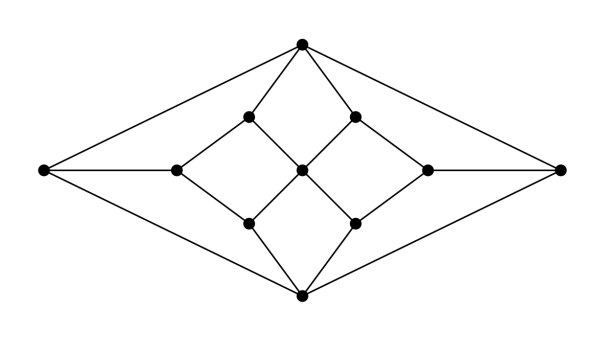
\includegraphics[width=7cm]{images/2.3.png}
    \end{center}
    
    \item \textit{(2 балла)} Имеется кусок проволоки длиной 12 сантиметров. На какое минимальное количество кусков его следует
    разрезать, чтобы из этих кусков можно было бы изготовить каркас кубика размерами $1\times1\times1$ при условии, что проволоку в процессе изготовления кубиков можно сгибать?
    
    \item \textit{(2 балла)} На поединок собрались $2n$ дуэлянтов. Некоторые пары дуэлянтов ненавидят друг друга, и это чувство всегда взаимно. Оказалось, что если какие-то два дуэлянта не ненавидят друг друга, то каждый из остальных ненавидит хотя бы одного из них, а кто-то ещё и обязательно ненавидит их обоих. Докажите, что всех дуэлянтов можно разбить на пары для дуэли так, чтобы каждая пара противников ненавидела друг друга.
    
    \item \textit{(2 балла)} Пусть $ab\notin E(G), d_G(a) + d_G(b)\geq v(G)$, а в графе $G + ab$ (т.е. графе, отличающемся от $G$ добавлением ребра $ab$) есть гамильтонов цикл. Докажите, что в графе $G$ также есть гамильтонов цикл.
    
\end{enumerate}
\end{document}
